\subsection{Approach Overview}

In this work we propose an automated approach for evaluating the UUX of software products by analyzing user reviews.
For the purpose of this work, a review is a piece of text detailing positive and negative aspects of a product, an overall assessment (rating) and recommendations for potential buyers, written by a user of the product. We concentrate on reviews written in dedicated websites, for example: Epinions \cite{Epinions},  Amazon \cite{Amazon}, US App Store \cite{AppStore} and Google Play \cite{GooglePlay}.  Figure \ref{fig:introduction_review_epinions} shows an example of a review extracted from the Epinions website.
 		\begin{figure}[ht]
		\raggedleft
  			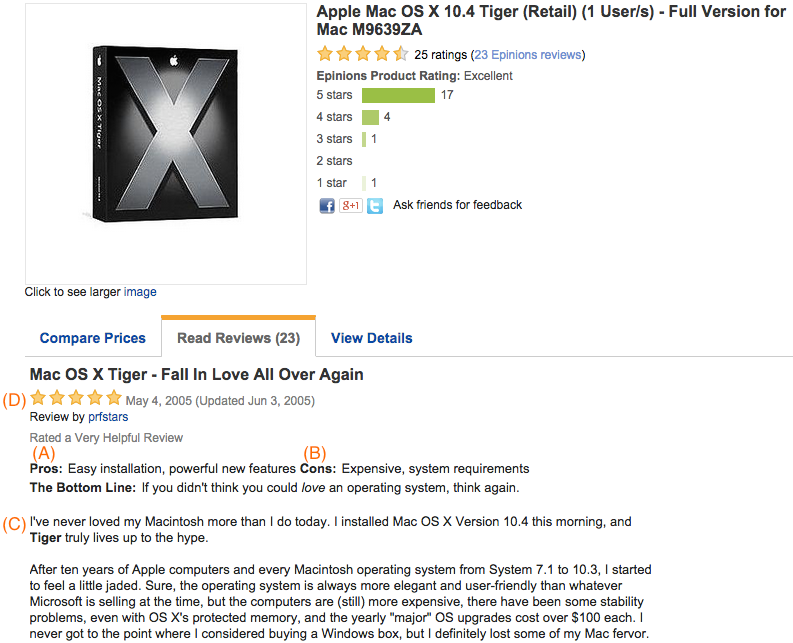
\includegraphics[width=0.4\textwidth]{img/introduction_review_epinions.png}
			\caption{Review example extracted from  Epinions website (28 January 2015). It details: (A) Positive aspects of the product, (B) Negative aspects of the product, (C) A general comment, (D) Overall assessment (rating).}
			\label{fig:introduction_review_epinions}
		\end{figure}

In this work, we propose a solution based on Natural Language Processing (NLP) techniques. NLP is a field of computer science, artificial intelligence, and linguistics concerned with the interactions between computers and human natural languages \cite{Bird2009}. One of the main applications of NLP involves natural language understanding, that is, enabling computers to derive meaning from human or natural language input.  This is our focus as our approach revolves around the analysis of written online reviews collected from dedicated review websites.  Specifically, we use machine learning techniques for UUX classification and sentiment analysis for determining the sentiment expressed in user reviews with regard to the product in general, or to features in particular. Fig \ref{fig:introduction_high_level_overall_approach_overview} depicts an overview our approach. 

		\begin{figure}[ht]
		\centering
  			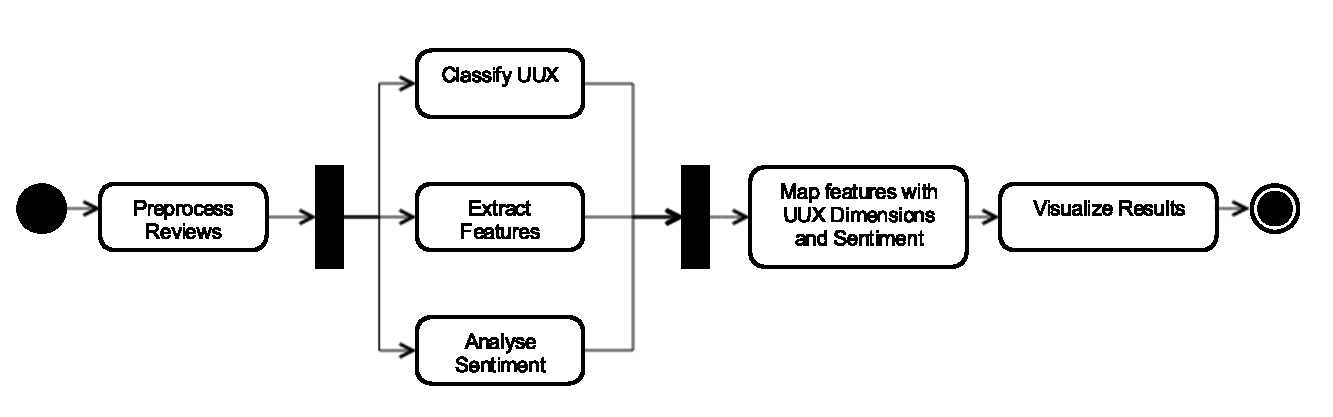
\includegraphics[width=0.4\textwidth]{img/introduction_acitvitydiagram_overallapproach.pdf}
			\caption{Overview of the approach (UML activity diagram).}
			\label{fig:introduction_high_level_overall_approach_overview}
		\end{figure}

One purpose of our approach is to provide an overall assessment of the sentiment of each UUX dimension, aggregated for the product in general, or fine-grained for each feature of the product. 
A UUX dimension can be a specific aspect, viewpoint, or phenomena within UUX (e.g., $Memorability$, $Satisfaction$, $Errors/Effectiveness$). A feature can be a description of specific software functionality (e.g., uploading files, sharing a link), a specific user interface (e.g., configuration screen, pdf viewer), a general quality of the software (e.g., price, privacy), as well as specific technical characteristics (e.g., encryption technology, multi-device syncing) \cite{Guzman2015}.
Our approach focuses on extraction of information from individual sentences, rather than entire reviews. As a review may incorporate both good and bad experiences relating to many different dimensions of UUX, a sentence-based bottom-up approach will yield more precise information about the ``typical" vocabulary associated to specific dimensions of UUX. By identifying the sentences that contain UUX information, we help the developers and UUX experts to filter the reviews by relevance and present only the most informative ones. 
Therefore, they can efficiently identify good and bad practices and gain insights on how to improve the product based on the users feedback.

\subsection{UUX Classification}

Initially, we construct a machine learning classifier that discriminates among dimensions based on words, or other features of the text that are automatically computed during the training of the classifier. The classifier automatically tags a sentence with the UUX dimensions it pertains to. This tagging task may be viewed as a set of binary classification tasks: for each dimension and each sentence, define whether the sentence relates to that dimension. 

For each UUX dimension, a binary machine learning classifier was trained and evaluated. Initially, the sentences were preprocessed, the data was split into five folds for performing cross-fold validation and then used for training the classifier. The feature vectors were weighted and ranked to discard the worst discriminating features. Finally, the SVM classifier was trained and standard performance measures were calculated.

\subsection{Sentiment Analysis}

The sentences containing UUX information are further analyzed and the expressed sentiment is detected. Similarly to the UUX classification, we use a machine learning classifier that categorizes each sentence as positive, neutral or negative. The approach is based on the hypothesis that people use specific words or phrases to express specific sentiments. Through the machine learning approach, the system can identify these 'keywords' and heavily rely on them for text classification. Furthermore, the system can learn how word phrases (e.g., bigrams) or punctuation are used to express specific sentiments.An unconventional step we took was negation handling. Hogenboom et al. \cite{Hogenboom2011} show that accounting for negation when analyzing sentiment in natural language texts helps improving the performance of classifying unseen natural language text as carrying either positive or negative sentiment. These results were also confirmed by our study. 

\subsection{Feature Extraction}

However, through the sentence level sentiment analysis we cannot understand what exactly users like or dislike about a product. User reviews not only express the overall sentiment about a specific product (e.g., ``This is a great  app"), but also sentiments related to its specific features, such as the functionality, performance, user interface, price etc. Subsequently, a review may convey opposing sentiments (e.g., ``Its performance is ideal, I wish I could say the same about the price") or objective information (e.g., ``You can adjust the volume, including normalizing all audio") for different features of a product.
Furthermore, the need for a fine grained analysis applies also to the UUX information. Users write their opinion about a product in general, however they can have different and even contradictory opinions about specific features of the product. 

\subsection{Merging of Classification, SA and Feature Extraction}


We perform a fine grained, feature level analysis as follows. Initially, the features are extracted and the feature sentiment is calculated as an average of the sentiment of the sentences that pertain to that particular feature. Similarly, the feature is mapped to all the UUX dimensions identified in sentences were the feature is present. For example, the sentence ``Still, it's a fun single player campaign, and a wonderful multiplayer experience"  is tagged by the UUX classifier with the following UXX dimensions: \textit{Hedonic, Pleasure, Affect/Emotion, Enjoyment/Fun}. The sentence level sentiment classifier tags the sentence as positive (fun, wonderful experience). The feature extraction process results in two features:  single-player campaign and multiplayer campaign. Finally, the two features are mapped with the sentence's UUX dimensions and sentiment as shown in Figure \ref{tab:example_results_approach}.

\begin{table}
\centering
\caption{The results of the approach for an example sentence: ``Still, it's a fun single player campaign, and a wonderful multiplayer experience".}
\label{tab:example_results_approach}
	\begin{tabularx}{\linewidth}{| p{4cm}|X| p{1.9cm}|}
	\hline
	\textbf{Features}&\textbf{UUX Dimensions}&\textbf{Sentiment}\\
	\hline
	Single-player Campaign&Hedonic, Pleasure, Affect/Emotion, Enjoyment/Fun&Positive\\
	\hline
	Multiplayer Campaign&Hedonic, Pleasure, Affect/Emotion, Enjoyment/Fun&Positive\\
	\hline
\end{tabularx}
\end{table}


\subsection{Visualization}

In the following paragraphs we introduce potential usage scenarios of the approach. 
Each usage scenario is supported by a visualization of the results (a report) that highlights specific aspects of the extracted information. The usefulness to the users, potentially developers and UUX experts (practitioners and researchers), is discussed for each usage scenario. 

In our main scenario, the user of the system gets an overview of the UUX sentiment on the most popular features of the system. The average sentiment of each UUX dimension across features and vice versa is visualized. In addition some of the most informative reviews for each UUX-feature pair are shown. These reviews are selected in such way that uniform distribution of review sentiment and rating is ensured.
Furthermore, users can search for particular features they are interested in and obtain the corresponding sentiment, the fine-grained sentiment for each UUX dimension and its most relevant reviews. Figure \ref{fig:introduction_scenario1} illustrates this scenario.
The purpose of this report is to provide a general overview of the sentiment of UUX dimensions across the most popular features. The users can easily identify the most 'problematic' features or UUX dimensions and further inspect them in the detailed reports described in the following paragraphs.


		\begin{figure}[ht]
		\raggedleft
  			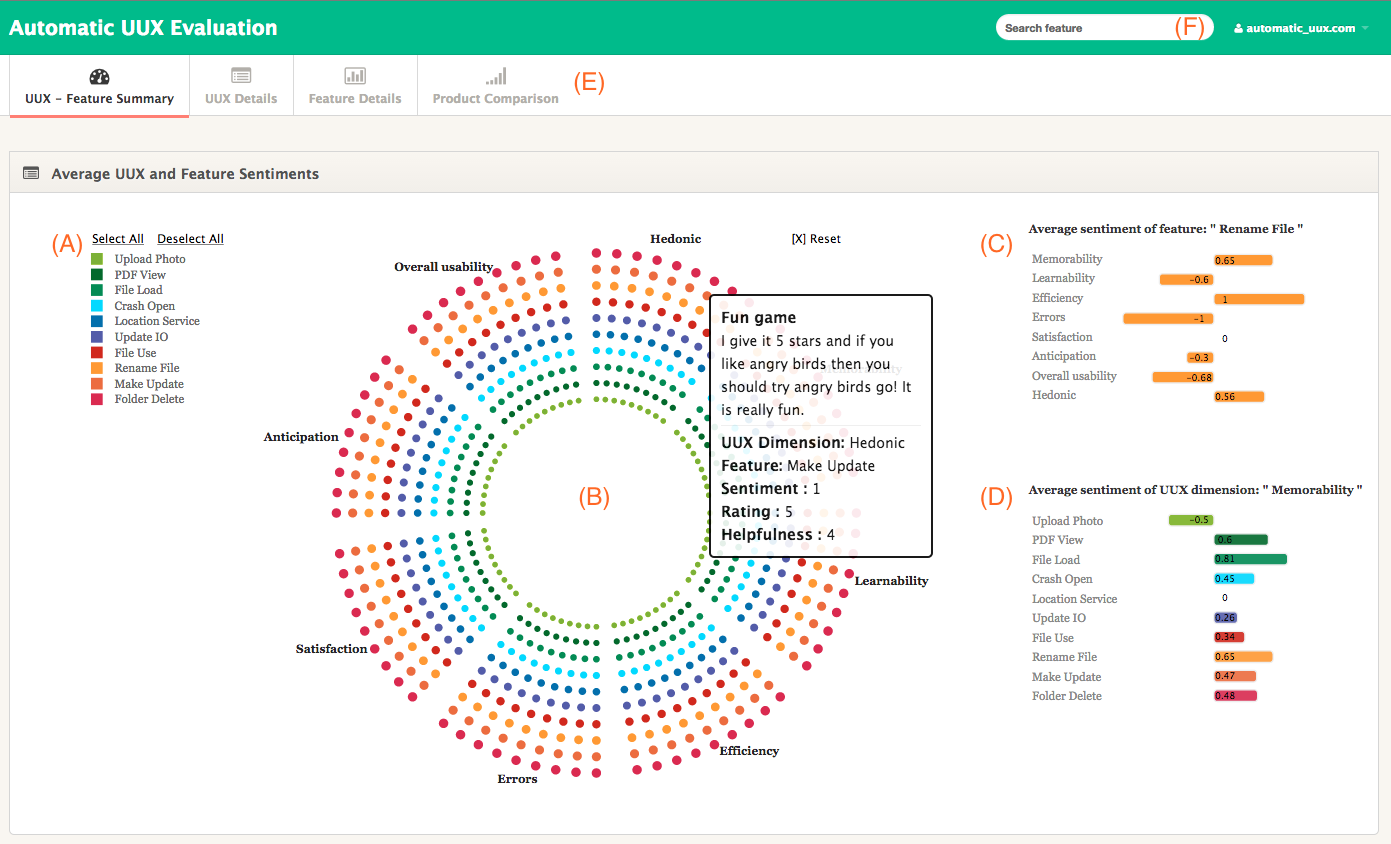
\includegraphics[width=0.4\textwidth]{img/introduction_scenario1.png}
			\caption{Feature-UUX overview. The following information is depicted in the view: (A) Most popular features (or the features the user has searched for), (B) Examples of some of the most relevant reviews for each UUX dimension-feature pair, (C) Average of the selected feature for each UUX dimension, (D) Average of the selected UUX dimension for each feature, (E) Navigation menu, (F) Search field to query features.}
			\label{fig:introduction_scenario1}
		\end{figure}

Another potential scenario is a fine-grained analysis of UUX.The average sentiments and the total number of reviews pertaining to each UUX dimension are depicted. The user can select a specific UUX dimension of interest and inspect the relevant user reviews over time, categorized based on the sentiment and rating. In addition, several statistics such as total number of reviews per sentiment level and average sentiment are shown (see Figure \ref{fig:introduction_scenario2}).
Initially, the visualized information is an aggregation over all features of the product. However, users can query for specific features they are interested in. 
A similar report would provide detailed information about the features of the product. The overall sentiment of the features or the sentiment with regard to specific UUX dimensions can be visualized. This report can be valuable especially to the development team by helping them identifying the most and least popular features and take decisions on how to improve them during software evolution.

		\begin{figure}[ht]
		\raggedleft
  			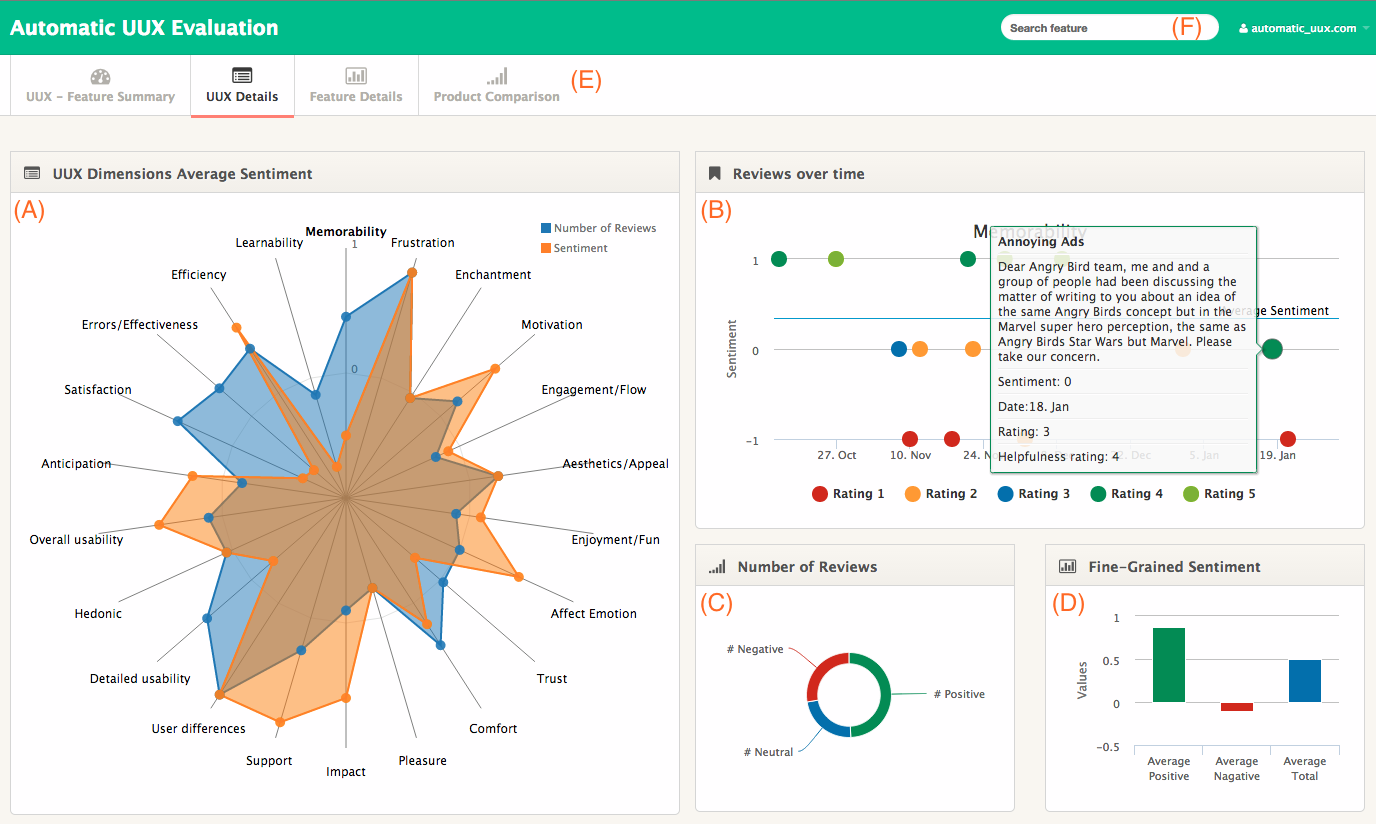
\includegraphics[width=0.4\textwidth]{img/introduction_scenario2.png}
			\caption{UUX Detailed View. The following information is depicted in the view: (A) Number of relevant reviews and average sentiment of each UUX dimension about the product in general (or about the features the user has searched for), (B) Reviews pertaining to the selected UUX dimension over time, (C) Number of positive, negative and neutral reviews pertaining to the UUX dimension, (D) Average positive sentiment, average negative sentiment and overall average sentiment of the selected UUX dimension, (E) Navigation menu, (F) Search field to query features.}
			\label{fig:introduction_scenario2}
		\end{figure}

Another potential usage scenario is the comparison of different products with respect to user sentiment on UUX. For example, by comparing products of a specific category (e.g., \textit{Evernote} and \textit{Note Everything}, two solutions for notetaking and archiving), with regard to specific features, the UUX experts can identify how design decisions are perceived by and influence users opinions (see Figure \ref{fig:introduction_scenario3}). Moreover, this report can be of particular interest to UUX researchers. They can identify good and bad UUX practices, study the applicability of the practices across different domains or across different user categories.

		\begin{figure}[ht]
		\raggedleft
  			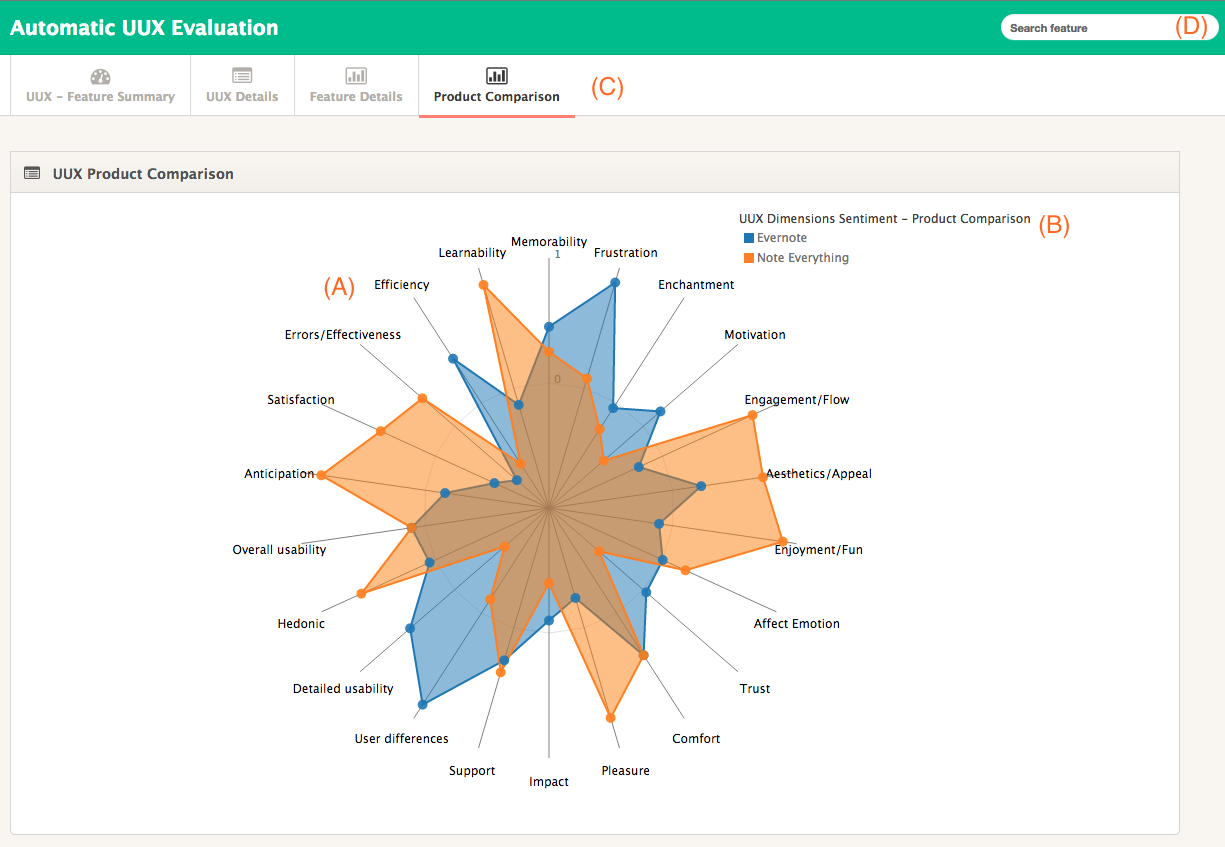
\includegraphics[width=0.4\textwidth]{img/introduction_scenario3.png}
			\caption{Product Comparison. The following information is depicted in the view: (A) Average sentiment of each UUX dimension for each of the products being compared, (B) General information (name, corresponding chart color) of the products, (C) Navigation menu, (D) Search field to query features.}
			\label{fig:introduction_scenario3}
		\end{figure}
